\chapter{Introducción}
\label{chapter:introduccion}

\section{Fundamentos}

En los últimos años ha habido un aumento considerable de datos de diversa índole
y generados por fuentes heterogéneas. Según los autores
\citeauthor{gantz_extracting_2011}, el volumen total de datos creados y
replicados en el mundo durante el año 2011 supera los 1.8 ZB (zettabytes) y se
ha estimado que duplica cada dos años \cite{gantz_extracting_2011}. Los avances
en el área de \acrfull{ti} han contribuido a una continua
producción de datos y expansión del campo digital, tal es el caso para la red
social \textit{Facebook}, la cual recibe cada hora un flujo de 10 millones de
fotos que publican sus usuarios \cite{mayer-schonberger_big_2013}. A estas
grandes colecciones de datos se las conoce como \textit{big data} y acarrean
nuevas oportunidades y desafíos al campo de las ciencias de la computación. En
cuestiones económicas, un análisis a gran escala en búsqueda de tendencias en el
comportamiento de los usuarios o clientes de un sistema puede dar una ventaja
competitiva en el mercado y, en adición, proveer de un servicio valioso a la
comunidad. Potencialmente, la \textit{big data} puede ser una fuente que
proporcione a la comunidad de conocimiento nuevo sobre el mundo en el que
habita, o como ha mencionado \citeauthor{fayyad_advances_1996} en su escrito
sobre el descubrimiento de conocimiento:

\begin{displayquote}
	\comillas{Los datos que percibimos de nuestro
		ambiente son la evidencia básica que usamos para construir teorías y modelos
		sobre el universo en el que vivimos}\footnote{\comillas{Data we capture about our
			environment are the basic evidence we use to build theories and models of the
			universe we live in} \cite[p. 2]{fayyad_advances_1996}. Traducción propia.}
\end{displayquote}

Sin embargo, volúmenes masivos de datos tornan obsoletos los tradicionales
métodos manuales de análisis de datos y surge la necesidad de desarrollar
técnicas automatizadas para extraer patrones en los datos y obtener
conocimiento. Con este fin, se han desarrollado técnicas en las áreas de minería
de datos y aprendizaje de máquinas que abordan estas colecciones en búsqueda de
conocimiento válido y útil. Dichas técnicas se han enfocado en el aprendizaje
por \textit{batch} \cite{gama_knowledge_2010}, lo que significa que el algoritmo
dispone de la colección completa, almacenada en disco, y con la cual genera un
modelo a partir de una o múltiples iteraciones sobre todos los datos. No
obstante, el aprendizaje por \textit{batch} trae aparejada una dificultad en su
misma definición: requiere de todos los datos de la colección presentes y
accesibles en todo momento,  lo cual no siempre es posible. Además, se suma una
limitante que es clave en el contexto actual de alta disponibilidad de datos:
hoy en día una buena parte de los datos generados proviene de flujos continuos o
\comillas{\textit{streamings}} de datos \cite{bifet_big_2014}. Estos flujos son
potencialmente ilimitados, arriban de a una instancia por vez, y son analizados
con restricciones altas de tiempo de procesamiento y de memoria.  Tal es el caso
para aplicaciones de sensores, monitoreo de redes y administración de tráfico,
flujo de clics de un usuario en la web, redes sociales, entre otros.  Los
algoritmos de aprendizaje que actúen en este entorno dinámico deben contar con
mecanismos que permitan manejar cambios en la naturaleza o distribución de los
datos, tanto para incorporar datos nuevos, como para descartar los datos
antiguos. Por estas razones, se torna necesario que las aplicaciones basadas en
clasificación en tiempo real adapten sus operaciones de entrenamiento y
predicción para lograr mejores resultados \cite{sousa_multi-label_2018}.

Dentro del área de minería de datos, una de las principales tareas es la de
clasificación, la cual consiste en entrenar un modelo que sea capaz de asignar
una única etiqueta a una instancia desconocida. No obstante, existen problemas
de clasificación en donde múltiples etiquetas son necesarias para caracterizar
una instancia. Por ejemplo, una noticia de diario referida al accidente aéreo
que sufrió el plantel de fútbol del club Chapecoense puede ser clasificado en la
categoría de \comillas{Fútbol} tanto como en la de \comillas{Tragedias}. Del
mismo modo, un video documental sobre la vida de Borges puede anotarse como
\comillas{Biografía}, \comillas{Literatura} o incluso \comillas{Buenos Aires} si
se mostraran imágenes de la ciudad. Este tipo de problemas es llamado
\acrfull{mll}\footnote{Siglas provenientes de su abreviación en inglés,
	Multi-label learning} y representa un nuevo paradigma de aprendizaje automático,
con sus propios retos por afrontar y que aún no ha sido suficientemente
explorado en proyectos de investigación.

Una clasificación multi-etiqueta permite conocer el grado de correlación entre
una instancia de la colección y una o más etiquetas. Esta cualidad significa un
mayor poder de generalización con respecto a la clasificación tradicional de
única etiqueta, ya que puede abarcar esos mismos problemas y otros de mayor
número de etiquetas. Además, existen algoritmos que aprovechan la correlación
entre etiquetas para mejorar la eficiencia de la clasificación y la calidad de
la predicción.

El campo de \acrshort{mll} se ha desarrollado considerablemente en los últimos
años, pero hasta el momento muchos de estos trabajos se han llevado a cabo en
ambientes estáticos de aprendizaje por
\textit{batch}~\cite{read_classifier_2011}, en consecuencia, se hace necesario
encarar nuevos proyectos que aborden clasificaciones \acrshort{mll} en contextos
de \textit{streaming} de datos. El desafío entonces consiste en crear
clasificadores que sean capaces de manejar un inmenso número de instancias y
adaptarse al cambio, a la vez que estar preparados para hacer tareas de
predicción en cualquier momento, y todo esto en un contexto de altas
restricciones de tiempo de respuesta y memoria.

\section{Descripción del Tema de Estudio}

\subsection{Clasificación Multi-etiquetas}
\label{intro_mll}

Tradicionalmente, el aprendizaje supervisado ha consistido en asociar una
instancia o ejemplo a una única etiqueta. Dicho ejemplo es una representación de
un objeto del mundo real, y por lo tanto, consta de características o atributos
particulares. La etiqueta corresponde a un significado semántico o concepto que
lo caracteriza. La tarea de clasificación entonces, reside en aprender una
función que permita enlazar ejemplos no observados con una etiqueta. Es preciso
notar aquí que dicha definición encubre la restricción de que cada instancia
pertenece a una única etiqueta, o dicho de otra manera, cada objeto del mundo
real se asocia a un único concepto y ningún otro. Sin embargo, existen problemas
de clasificación donde más de una etiqueta puede ser asignada a un ejemplo. La
anterior presunción no se amolda a problemas complejos donde un objeto pueda
tener más de un significado simultáneamente.

Tareas de este tipo pueden surgir en áreas como las de categorización de texto,
recuperación de información musical, clasificación semántica de escenas,
anotación automática de videos o  clasificación de genes y funciones proteicas.
A modo de ejemplo, en el campo mencionado de clasificación semántica de escenas,
la foto de un paisaje que ilustra una montaña y una playa puede asociarse a las
categorías de ‘playa’ y ‘montaña’, simultáneamente \cite{gibaja_tutorial_2015};
en bioinformática, cada gen puede ser asociado a clases según su función, tales
como ‘metabolismo’, ‘transcripción’ o ‘síntesis proteica’
\cite{zhang_multi-label_2010}; por último, en recuperación de información
musical una pieza sinfónica puede tener \textit{tags} como ‘Mozart’, ‘piano’ o
‘clásica’.

Este nuevo paradigma es llamado '\acrlong{mll}'   y ataca problemas con las
siguientes características \cite{gibaja_tutorial_2015}:

\begin{itemize}

	\item El conjunto de etiquetas es previamente definido y tiene un significado
	      interpretable por un humano.

	\item El número de etiquetas es limitado y no mayor que el número de
	      atributos.

	\item En caso de que el número de atributos sea grande, se debe poder aplicar
	      estrategias de reducción de atributos.

	\item El número de ejemplos puede ser grande.

	\item Las etiquetas pueden estar correlacionadas. Esto significa que se
	      pueden aplicar técnicas que exploten estas relaciones con el objetivo de
	      reducir los tiempos de procesamiento de los algoritmos.

	\item La distribución de los datos puede estar desbalanceada, es decir, que
	      una etiqueta puede tener un mayor número de ejemplos que otras.

\end{itemize}

Asimismo, surge un desafío a superar: el conjunto de etiquetas posible crece
exponencialmente ante cada nueva adición de una etiqueta. Por ejemplo, si se
tuvieran 20 etiquetas, la cantidad posible de conjuntos de etiquetas distintos
excedería el millón (\(2^{20}\)). Esto implica un tamaño exorbitante del espacio
de salida y, en consecuencia, costos computacionales altos. En ese sentido, se
ha buscado desarrollar algoritmos que aprovechan las correlaciones o
dependencias entre etiquetas. Por ejemplo, la probabilidad de que una noticia
que contiene los términos ‘pelota’ y ‘gol’ sea anotada con la etiqueta ‘fútbol’
sería mayor que si se etiquetara con la etiqueta ‘tenis’.
\citeauthor{zhang_multi-label_2010} clasifican estos algoritmos en tres grupos
según la estrategia de correlación aplicada \cite{zhang_multi-label_2010}:

\begin{description}
	\label{estrategias_mll}

	\item[Estrategia de primer orden] La tarea de \acrshort{mll} es dividida en
	      $q$ tareas de clasificación binarias, siendo $q$ el número de etiquetas de
	      la colección.

	\item[Estrategia de segundo orden] La tarea de \acrshort{mll} se basa en la
	      generación de relaciones de a pares de etiquetas ya sea por
	      \textit{rankings} entre clases relevantes y no relevantes o por
	      interacción entre pares de etiquetas.

	\item[Estrategia de alto orden] La tarea de \acrshort{mll} considera
	      relaciones de alto orden entre etiquetas.

\end{description}

Las estrategias de primer orden son conceptualmente simples y eficientes pero
logran resultados de menor calidad porque no consideran correlaciones. Las
estrategias de segundo orden tienen un mayor poder de generalización pero no
todos los problemas de \acrshort{mll} pueden ser abarcados. El último grupo, por
su parte, modela las correlaciones más potentes, pero conlleva un costo
computacional alto.

En el último tiempo, muchos son los algoritmos que han sido desarrollados para
atacar el problema de la clasificación \acrshort{mll}. La comunidad de
investigación ha aceptado la taxonomía definida por
\citeauthor{tsoumakas_multi-label_2007}, para estudiar y clasificar los
distintos algoritmos de la literatura \cite {gibaja_tutorial_2015}. La misma
propone dos grandes grupos:

\begin{description}

	\item[Métodos de transformación del problema] Este tipo de algoritmos
	      transforman el problema de clasificación \acrshort{mll} en un problema de
	      clasificación tradicional. Ejemplos típicos de este grupo son \acrfull{br}
	      \cite{tsoumakas_multi-label_2007} y \acrfull{cc}
	      \cite{read_classifier_2011}. Ambos convierten la tarea en una de
	      clasificación binaria.

	\item[Métodos de adaptación del algoritmo] Son algoritmos que toman métodos
	      tradicionales de aprendizaje, como árboles de decisión o \textit{naive
		      bayes}, y los adaptan a la tarea de clasificación \acrshort{mll}.

\end{description}

A modo ilustrativo, la figura~\ref{fig:algorithm_taxonomy} es un diagrama de la
taxonomía de algoritmos confeccionado por \citeauthor{zhang_review_2014} \cite
{zhang_review_2014}.

\begin{figure}
	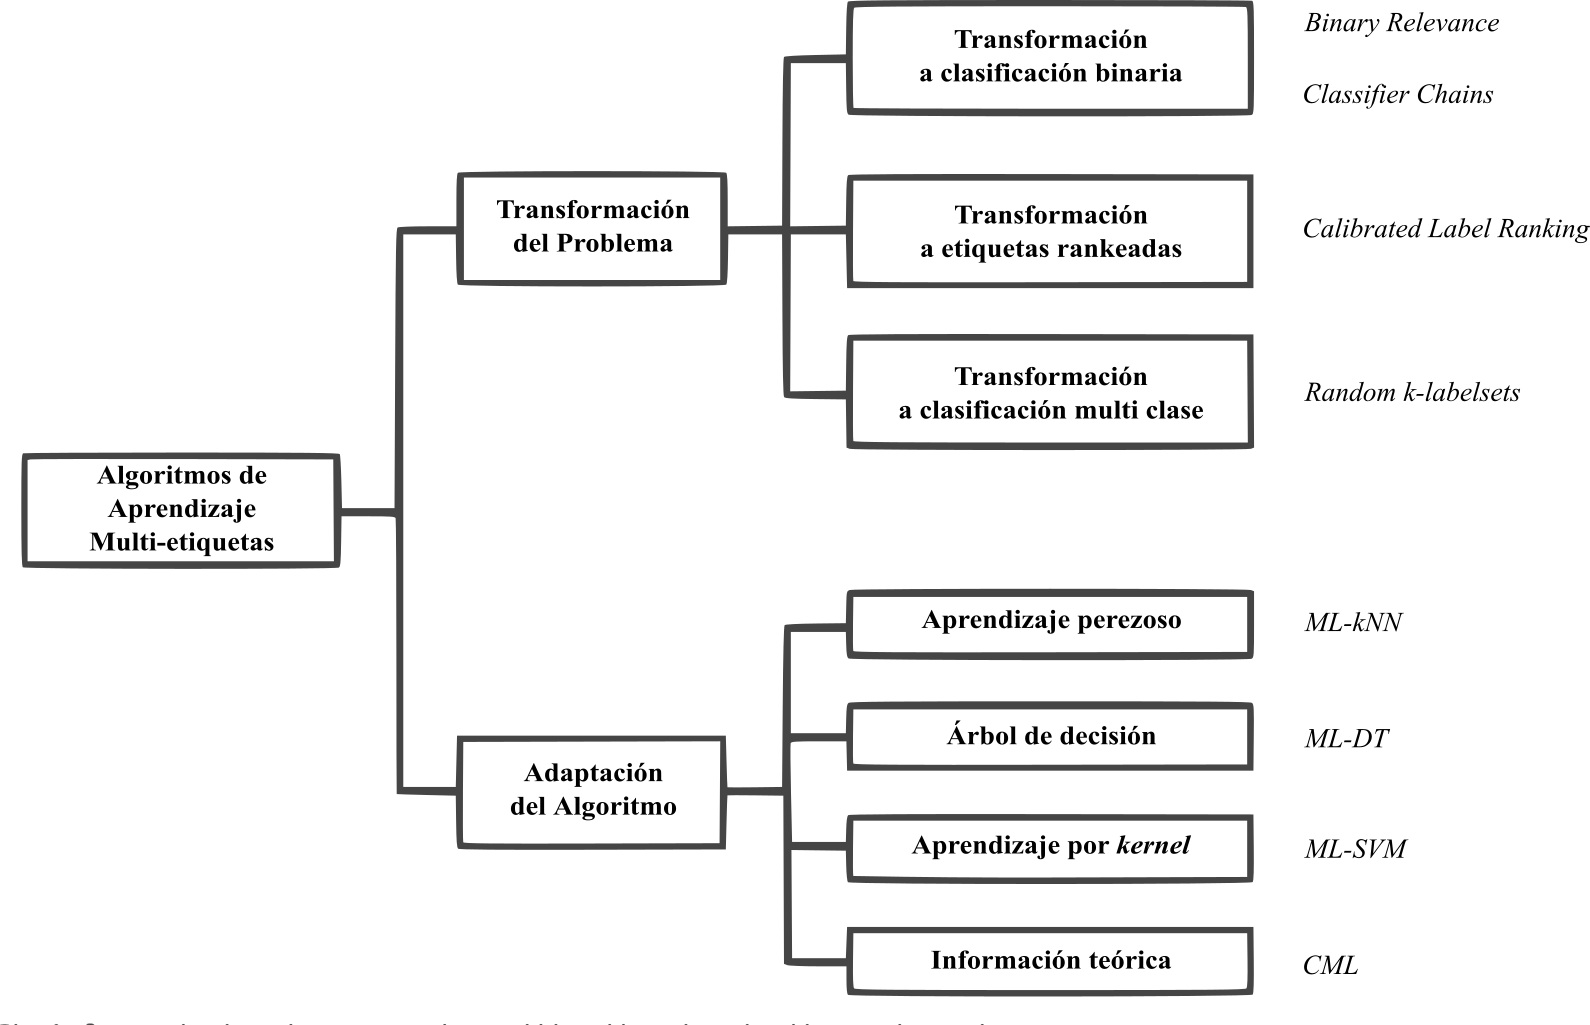
\includegraphics[width=\linewidth]{figures/algorithm_taxonomy.png}
	\caption{Categorización de los algoritmos de \acrshort{mll} más representativos.}
	\label{fig:algorithm_taxonomy}
\end{figure}

\subsection{Flujos Continuos de Datos}
\label{intro_streams}

Hoy en día, los datos pueden ser generados por elementos de continuo monitoreo
del medio, tales como sensores o archivos de registro.  La clasificación de
flujos continuos de datos o \textit{streamings} se enfoca en problemas de este
tipo, en donde objetos del mundo real son analizados en tiempo real. Un
\textit{stream} se considera como una secuencia ordenada de datos que fluye a
alta velocidad y es teóricamente infinita. A continuación se describe brevemente
las características de este tipo de datos y los requisitos que debe cumplir un
algoritmo para poder tratar con ellos.

\subsubsection{Características}
\label{stream_caracteristicas}

En escenarios de \textit{streamings}, los datos deben cumplir con las siguientes
características \cite {gama_knowledge_2010}:

\begin{itemize}

	\item Los datos están disponibles a través de flujos continuos e ilimitados
	      en el tiempo, a diferencia del aprendizaje por \textit{batch} donde los
	      datos son acotados.

	\item Las regularidades subyacentes de los datos no son estacionarias, sino
	      que pueden evolucionar. En otras palabras, la distribución de los datos es
	      susceptible a cambios en el tiempo.

	\item La data ya no es considerada independiente e idénticamente distribuida.

	\item La data está situada tanto en el espacio como en el tiempo. La lectura
	      y procesamiento de los datos debe ser lo suficientemente veloz como para
	      procesar el siguiente dato, de otro modo, el dato ya no podrá ser procesado
	      en el futuro.

\end{itemize}

\subsubsection{Requisitos de los algoritmos}
\label{stream_requisitos}

Para hacer frente a estas características de los datos, los sistemas o
algoritmos deben contar con los siguientes requisitos \cite{hulten_mining_2001}:

\begin{itemize}

	\item El tiempo para procesar cada registro debe ser constante y pequeño.

	\item Debe usar un tamaño fijo de memoria principal y no dependiente de la
	      cantidad de registros ya procesados.

	\item El modelo es generado a partir de una única pasada sobre los datos.

	\item Debe contar con un modelo listo para realizar predicciones en cualquier
	      momento.

	\item Idealmente, deberá producir un modelo equivalente o casi idéntico al que
	      hubiera sido producido en un ambiente de \textit{batch}.

	\item Debe mantenerse actualizado ante evoluciones o derivas de concepto en
	      los datos.

\end{itemize}

Los algoritmos que cumplen con estas cualidades son llamados algoritmos de
aprendizaje adaptativo y, aplicados a tareas de clasificación como el de
multi-etiquetas, pueden aprovecharse para entrenar un mayor número de objetos y
predecir en cualquier instante.


\section{Motivación}

Ante la necesidad de hacer frente a un contexto global de generación masiva de
datos y a ritmo acelerado, se hace preciso fortalecer las técnicas de
aprendizaje automático actualmente presentes en el campo. En este escenario ya
no es posible contar con todos los datos almacenados físicamente y la idea de
generar un modelo completo para luego evaluarlo en una fase posterior debe ser
reemplazada por una en donde el modelo esté siempre listo para realizar
predicciones y al mismo tiempo ser capaz de reentrenarse y recalcular las
métricas de evaluación ante cada nueva instancia abordada. Todo esto en un
contexto cambiante, de alta disponibilidad y de limitación en el espacio de
almacenamiento. Si bien existen métodos de clasificación para flujos continuos
que han dado resultados satisfactorios, aún es un campo conveniente de ser
abordado. Asimismo, reproducir los experimentos realizados y fortalecer las
técnicas y herramientas actuales puede ser beneficioso para lograr estudios
precisos y pormenorizados que sean valiosos tanto para la comunidad científica
en sí misma, como también para la sociedad en general.

Por otro lado, si bien existen en el mundo real infinidad de datos
multi-etiquetados aún no es posible hallar colecciones disponibles al público
que cuenten con todas las características de un flujo continuo de datos. Uno de
los enfoques abordados es convertir las colecciones existentes en flujos tales
que arriben en conjuntos predefinidos y a lo largo del tiempo. De esta manera
los algoritmos pueden ser utilizados para realizar clasificaciones en un
ambiente similar al de un escenario de \textit{streaming}. Sin embargo, estas
colecciones tienen un número limitado de instancias y, por lo tanto, no cumplen
con la condición de ser teóricamente infinitos. Es entonces aquí donde surgen
las técnicas de generación sintética de instancias, que buscan reproducir la
distribución subyacente de los datos para simular colecciones de datos del mundo
real. La contracara de este enfoque es que, si bien existen técnicas y
herramientas para generar datos etiquetados, buena parte de ellos son solo
aplicables para instancias de una única etiqueta y los que logran generar datos
multi-etiquetados no han sido lo suficientemente explorados en el área. Hasta el
momento, los generadores de instancias multi-etiquetadas son capaces de generar
datos cercanos a los de colecciones del mundo real \cite{read_generating_2009} y
brindan la posibilidad de realizar estudios relativamente certeros de algoritmos
de clasificación \cite{read_scalable_2012}. No obstante, debe notarse también
que si bien se han obtenido colecciones sintéticas en sí mismas aún no han
logrado generar instancias para una colección en concreto, respetando sus
cualidades particulares y que las distinguen de otras, tales como la
co-ocurrencia de etiquetas, la densidad y cardinalidad de las etiquetas y la
relación entre las etiquetas y sus atributos, por mencionar algunas. De lograr
esta aproximación se podrán realizar estudios sobre el impacto de los algoritmos
sobre flujos de datos de naturaleza distintiva, o en otras palabras, entender en
qué medida un algoritmo es más apropiado que otro para un conjunto de datos en
un determinado contexto.

Esta última idea mencionada, es decir, el ser capaz de hallar las fortalezas y
debilidades de un algoritmo de \acrshort{mll} en un contexto determinado es
clave para evaluar la clasificación y entender los resultados obtenidos.
Estudios como el de \citeauthor{sousa_multi-label_2018}
\cite{sousa_multi-label_2018} o el de \citeauthor{read_scalable_2012}
\cite{read_scalable_2012} se han topado con que algoritmos de menor complejidad
pueden ser competitivos o incluso superar las métricas de otros algoritmos más
complejos. Esta variabilidad en los resultados no solo contrae la necesidad
antes mencionada de realizar más estudios al respecto, sino que también abre las
puertas a incursionar en soluciones de ensambles de algoritmos. Estos ensambles
han dado probada muestra de potenciarse ante la diversidad de resultados
obtenidos por sus estimadores base \cite{polikar_polikar_2006}, ya que son
capaces de disminuir el error total mediante estrategias combinativas. De
cualquier manera, las estrategias de ensamble existentes para flujos continuos
no han recibido la misma atención que aquellas aplicadas sobre ambientes de
\textit{batch} y queda mucho camino por recorrer.



\section{Objetivos}
\label{intro_objetivos}

El objetivo principal es estudiar el impacto de distintos algoritmos de
clasificación sobre datos multi-etiquetados en ambientes de \textit{streaming} y
provenientes de fuentes de distinto origen y naturaleza, en particular se
seleccionan colecciones de datos que son puntos de referencia en la literatura y
que poseen características distintivas entre sí, tales como el número de
etiquetas, el número de atributos, o la cantidad de instancias. A su vez, es
necesario convertir estos datos a flujos continuos. A este fin se generan
instancias sintéticas que sean fieles a estas características mencionadas,
aplicando técnicas existentes pero también extendiéndolas para detectar
co-ocurrencias entre etiquetas. De esta manera, se buscan obtener
representaciones óptimas de las colecciones. Por otro lado, se llevarán a cabo
clasificaciones con algoritmos clásicos y con soluciones de ensambles, en
búsqueda de maximizar los valores de las métricas de evaluación en cada
escenario. En este sentido, se diseñan distintas configuraciones de ensambles,
variando los estimadores base y probando distintas implementaciones. A este fin,
se diseña y desarrolla una nueva versión de algoritmo de votación por mayoría,
llamado \acrshort{efmp}, y se compara su rendimiento contra otros algoritmos de
\acrshort{mll} bien conocidos.

En resumen, se listan a continuación los objetivos particulares del trabajo:

\begin{itemize}

	\item \sout{Obtener colecciones de datos que cumplan con las propiedades
		      requeridas para considerarse un flujo continuo. Las características
		      deben variar entre colecciones.}

	\item Generar flujos continuos de datos a partir de la colección
	      proporcionada buscando replicar su número de etiquetas, atributos e
	      instancias, su cardinalidad y densidad de etiquetas y la co-ocurrencia
	      entre dos etiquetas. Aplicar técnicas conocidas de generación de
	      instancias sintéticas, proponer una técnica nueva y comparar los
	      resultados.

	\item \sout{Ejecutar algoritmos de clasificación de \acrshort{mll}, para
		      obtener modelos y realizar evaluaciones sobre los resultados. Todo esto
		      sobre distintos escenarios de flujos continuos.}Evaluar la capacidad
	      predictiva de los principales algoritmos de MLL sobre diferentes escenarios
	      de flujos continuos.

	\item \sout{Proponer una solución de ensambles a partir de la combinación de
		      algoritmos seleccionados de la literatura.}Desarrollar y evaluar una
	      solución de MLL basada en ensamble a partir de algoritmos clásicos del
	      área de estudio.

\end{itemize}


\section{Aportes}

El presente  trabajo de investigación aborda el campo de aprendizaje por
multi-etiquetas a partir de la experimentación y evaluación de técnicas y
algoritmos de la literatura sobre colecciones de naturaleza cambiante.
\acrshort{mll} es un paradigma emergente de aprendizaje supervisado cuyas
características implícitas abren paso a nuevos desafíos que derivan del
crecimiento exponencial de etiquetas y sus combinaciones, y del costo
computacional de entrenar y consultar el modelo. También suelen presentarse
otras propiedades como la alta dimensionalidad, data evolutiva y desbalanceada o
dependencia entre etiquetas, las cuales implican una resignificación de las
técnicas y métodos tradicionales del área de minería de datos.

El paradigma de \acrshort{mll} ha dado muestras de su eficiencia en términos de
tiempos de configuración y ejecución de las tareas, bajo diversos campos de
aplicación tales como los de categorización de texto, diagnósticos médicos,
minería de redes sociales o análisis de datos químicos, y se mantiene en
constante expansión hacia nuevos dominios de aplicación. Asimismo, su continua
integración a problemas de diversa naturaleza ha contribuido a alimentar esta
tendencia.

La tarea de clasificación de \textit{streaming} de datos se enfoca en problemas
donde objetos del mundo real son generados y procesados en tiempo real. Datos de
este tipo, y que además poseen múltiples etiquetas, son frecuentes en escenarios
del mundo real tal como sitios de publicación de imágenes, correos electrónicos
o portales de noticias. Abordar este tipo de problemas implica que los
algoritmos sean capaces de identificar cambios de concepto en los datos y
adaptarse al nuevo contexto. De lograr esto, se podrá generar modelos más
sólidos, ya que se cuenta con un mayor número de objetos, y que se encontrarán
aptos para predecir en cualquier momento. Surge entonces el reto de crear
clasificadores que actúen en ambientes de altas restricciones computacionales y
sean capaces de manejar un inmenso número de instancias, lidiar con evoluciones
en los datos y estar listos para resolver tareas de predicción en tiempo real.

A diferencia de otros trabajos de investigación recientes, este proyecto lleva a
cabo estudios experimentales sobre el tema de clasificaciones multi-etiquetas,
para hallar las fortalezas y debilidades de distintos algoritmos de aprendizaje
sobre distintos tipos de colecciones, con miras a aportar de un mayor
conocimiento empírico sobre el tema a la comunidad científica especializada en
tareas de clasificación de flujos de datos multi-etiquetados. El presente
trabajo espera contribuir al estudio de métodos y técnicas asentadas, pero
también examinar algoritmos exitosos del campo de aprendizaje por
\textit{batch}, particularmente los de ensambles de estimadores, a fin de
extender su funcionalidad a ambientes de flujos continuos, analizar su desempeño
y determinar en qué medida son aptos o no para este tipo de ambientes.


\section{Organización del Trabajo}

El presente escrito de tesis sigue la estructura clásica de proyecto de
investigación aplicado. Para comenzar, se brinda el marco teórico en el que se
sitúa el trabajo (capítulo~\ref{chapter:preliminares}), luego se describe la
metodología a seguir (capítulo~\ref{chapter:metodologia}), se presentan los
experimentos y sus resultados (capítulo~\ref{chapter:experimentos}), y
finalmente, se trazan las conclusiones arribadas y las futuras líneas de
investigación (capítulo~\ref{chapter:conclusiones}). A continuación, se describe
con más detalle cada capítulo del escrito:

\begin{description}

	\item{Capítulo~\ref{chapter:preliminares}. \nameref{chapter:preliminares}}:
	      En este capítulo se sitúa el trabajo dentro del campo de estudio general
	      y se introducen los conceptos claves, tanto de la tarea de clasificación
	      multi-etiquetas como también de los ambientes de flujos continuos, para
	      comprender los subsecuentes capítulos. La sección de clasificación
	      \acrshort{mll} cuenta con una definición formal de la tarea, presenta
	      los tipos de algoritmos existentes, junto con algunos de sus principales
	      exponentes y describe métricas de evaluación utilizadas para evaluar los
	      resultados de la clasificación.  Posteriormente, se da una descripción
	      detallada del concepto de flujo continuo y se extienden los conceptos
	      presentados de \acrshort{mll} para contextos de este tipo.

	\item{Capítulo~\ref{chapter:metodologia}. \nameref{chapter:metodologia}}: En
	      este capítulo se describe la metodología aplicada para entrenar y
	      clasificar modelos de \acrshort{mll} en ambientes de \textit{streaming}
	      así como también la generación y análisis de datos sintéticos. A su vez,
	      se exponen las técnicas propuestas que son propias y originarias de este
	      trabajo, lo que incluye, por un lado, un método que provee una serie de
	      parámetros para generar datos sintéticos a partir de una colección dada
	      y, por otro, una nueva solución de ensambles de votación por mayoría.

	\item{Capítulo~\ref{chapter:experimentos}. \nameref{chapter:experimentos}}:
	      En este capítulo se emprende la definición de los experimentos,
	      incluyendo las colecciones de datos y los algoritmos seleccionados para
	      la evaluación, así como también el hardware y software utilizado. Luego
	      se exponen los resultados, incluyendo tablas y gráficos que facilitan la
	      observación y comparación entre escenarios. Para los experimentos
	      concernientes a la generación sintética, se estudian los fenómenos de
	      colecciones multi-etiquetas y su aparición en los nuevos datos. Para los
	      experimentos de evaluación de algoritmos, se analizan los resultados de
	      cada métrica de evaluación para las pruebas ejecutadas en nuestro
	      ambiente y luego se comparan contra los resultados de otros autores de
	      la literatura en sus respectivos escritos.

	\item{Capítulo~\ref{chapter:conclusiones}. \nameref{chapter:conclusiones}}:
	      En este capítulo se abordan las conclusiones obtenidas una vez
	      desarrollados los objetivos y presentado los resultados, y se definen
	      las líneas de investigación futuras.

\end{description}
